%! suppress = SentenceEndWithCapital
%! suppress = LineBreak
%! suppress = Unicode
%! suppress = MissingLabel
%! suppress = MissingImport
%! suppress = FileNotFound
\documentclass[../main.tex]{subfiles}

\begin{document}

    \subsection{Jakość oprogramowania}
    Jakości jest pojęciem \textbf{niejednoznacznym} i \textbf{wielowymiarowym}.

    \textbf{Różne spojrzenia wg Garvina:}
    \begin{itemize}
        \item jakość oparta na \textbf{produkcie} (np. charakterystyki jakościowe)
        \item jakość oparta na \textbf{użytkowniku} (funkcjonalność, fitness for use)
        \item jakość oparta na \textbf{wytwarzaniu} (jakość „techniczna” procesu)
        \item jakość oparta na \textbf{wartości} (czas vs. wysiłek vs. koszt)
        \item jakość \textbf{transcendentna} (nieoperacyjna, trudno mierzalna, np. „grywalność” gry komputerowej)
    \end{itemize}

    \subsubsection{Model jakości ISO 9126}

    \begin{table}[H]
        \begin{center}
            \begin{tabular}{ p{8cm} p{8cm}}
                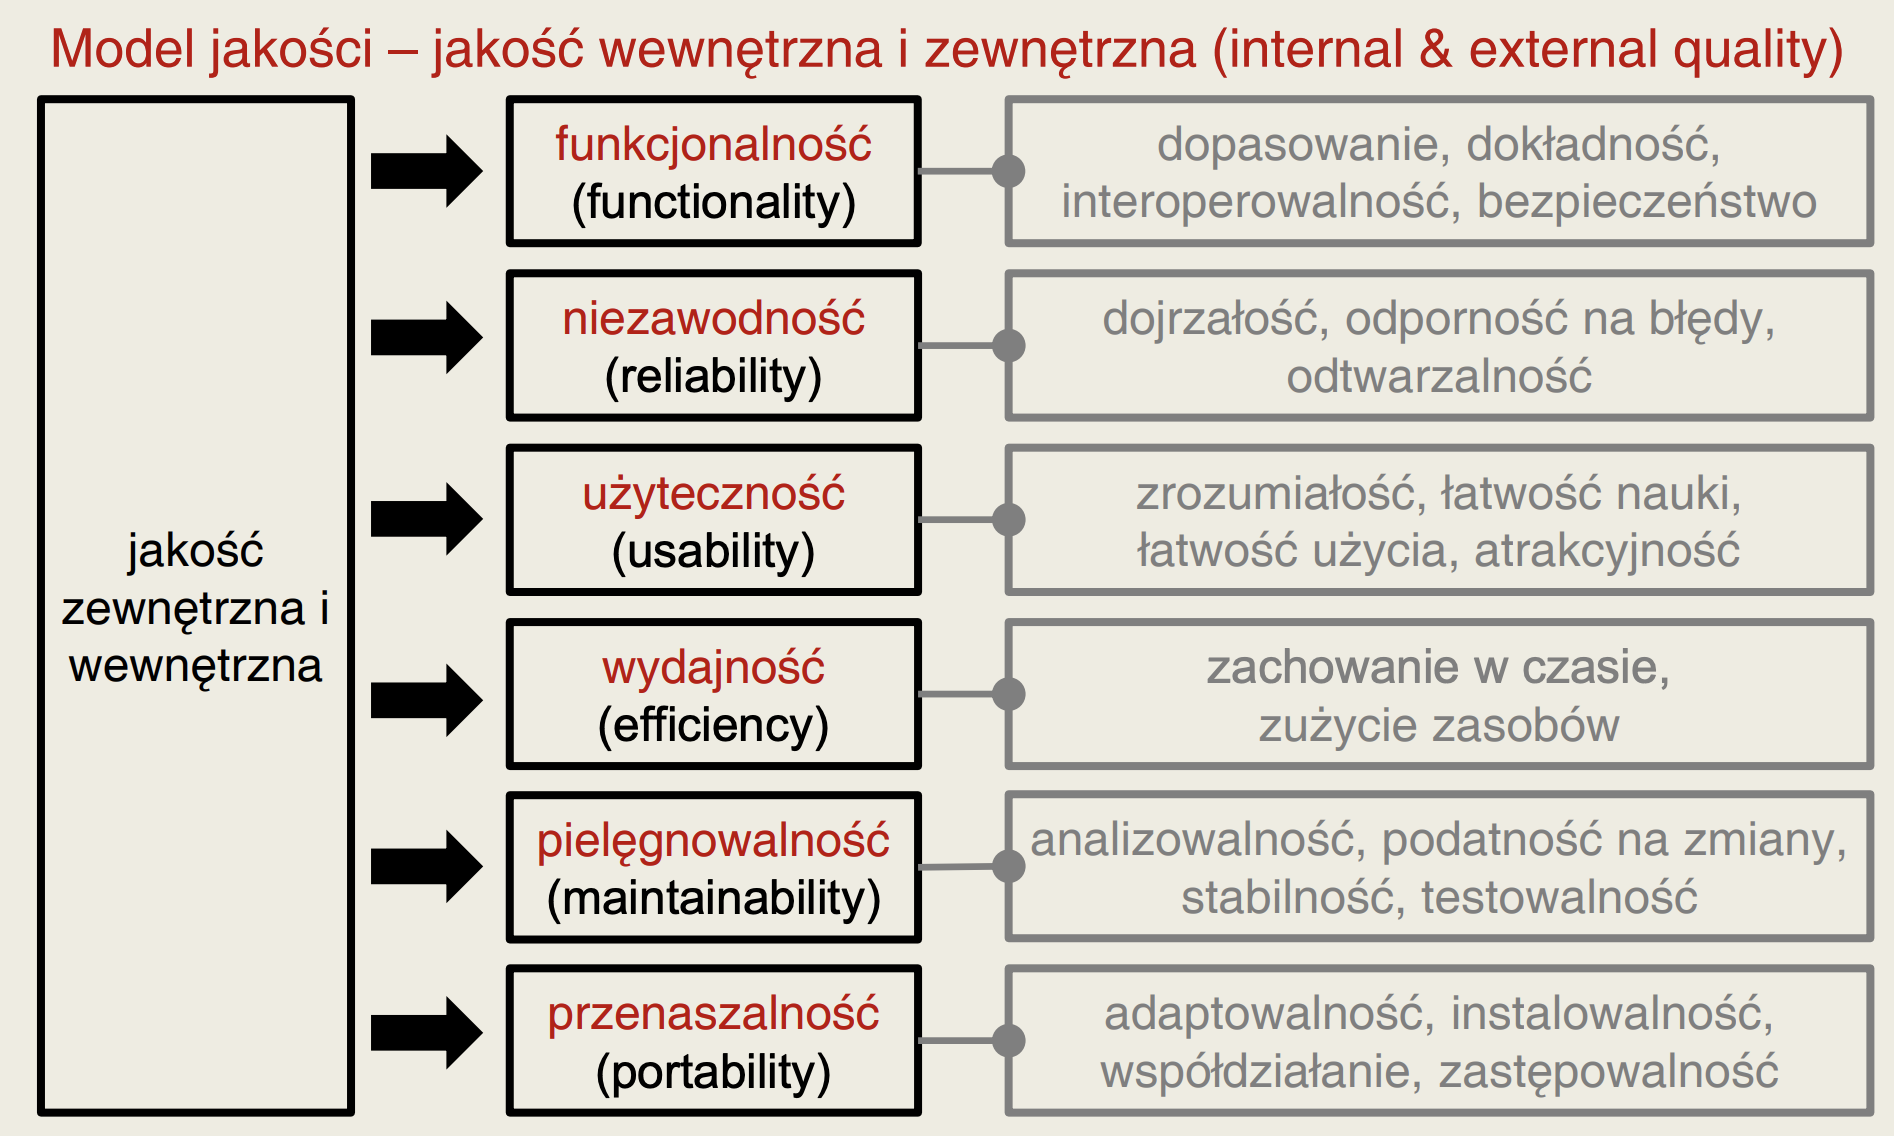
\includegraphics[width=8cm]{ISO9126_1.png}
                &
                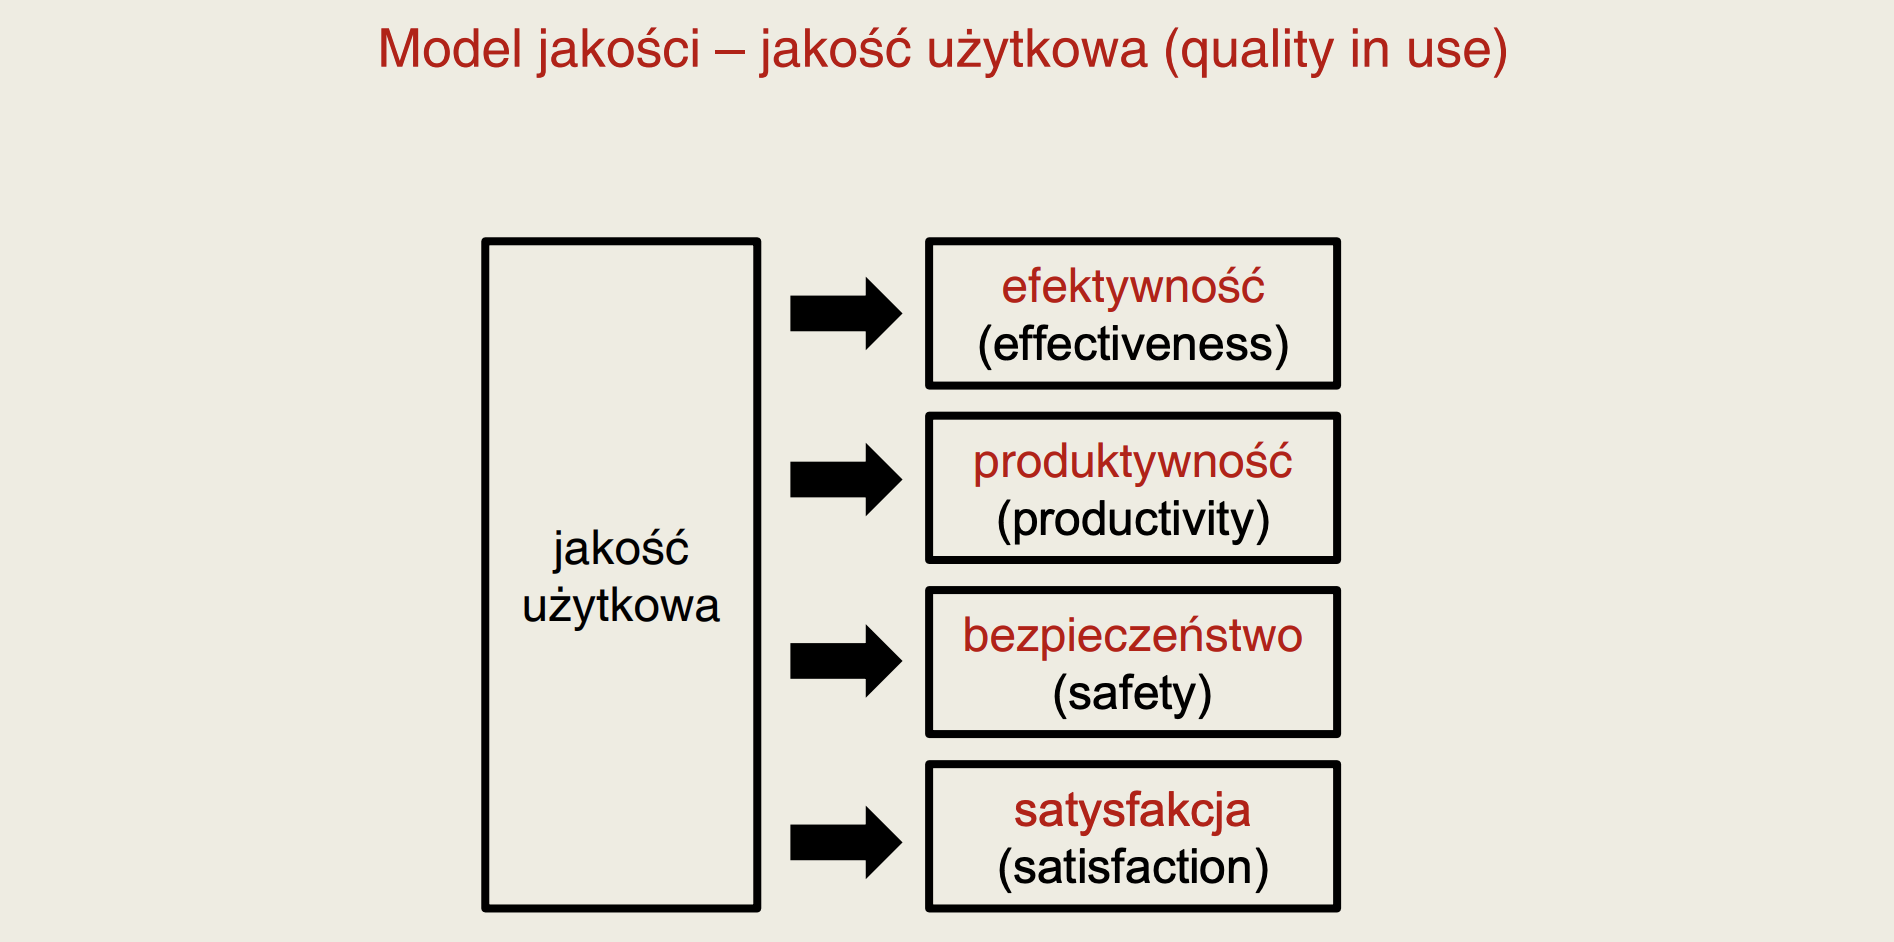
\includegraphics[width=8cm]{ISO9126_2.png}
            \end{tabular}
        \end{center}
    \end{table}

    \subsubsection{Model jakości ISO/IEEE 25000}
    Nowa rodzina norm, zastępująca starą normę 9126.

    \begin{table}[H]
        \begin{center}
            \begin{tabular}{p{8cm} p{8cm}}
                \textbf{ Jakość produktu} (system/software product quality):
                \begin{itemize}
                    \item funkcjonalna przydatność
                    \item wydajność w działaniu
                    \item zgodność
                    \item użyteczność
                    \item niezawodność
                    \item bezpieczeństwo
                    \item pielęgnowalność
                    \item przenaszalność
                \end{itemize}
                &
                \textbf{Jakość użytkowa} (quality in use)
                \begin{itemize}
                    \item efektywność
                    \item wydajność
                    \item satysfakcja
                    \item wolność od ryzyka
                    \item kontekst użycia
                \end{itemize}
            \end{tabular}
        \end{center}
    \end{table}

    \subsubsection{Niezawodność}

    \textbf{Niezawodność} - \textbf{zdolność} oprogramowania do \textbf{bezbłędnego działania} przez określony czas lub przez określoną
    liczbę operacji.

    Testy niezawodności wykorzystują \textbf{profile operacyjne}.

    \textbf{Cechy niezawodności}:
    \begin{itemize}
        \item \textbf{dojrzałość} (zdolność do bezawaryjnego działania przy występowaniu usterek)
        \item \textbf{tolerancja na błędy} (np. obsługa wyjątków)
        \item \textbf{odtwarzalność} (zdolność działania po awarii)
    \end{itemize}

    \begin{figure}[H]
        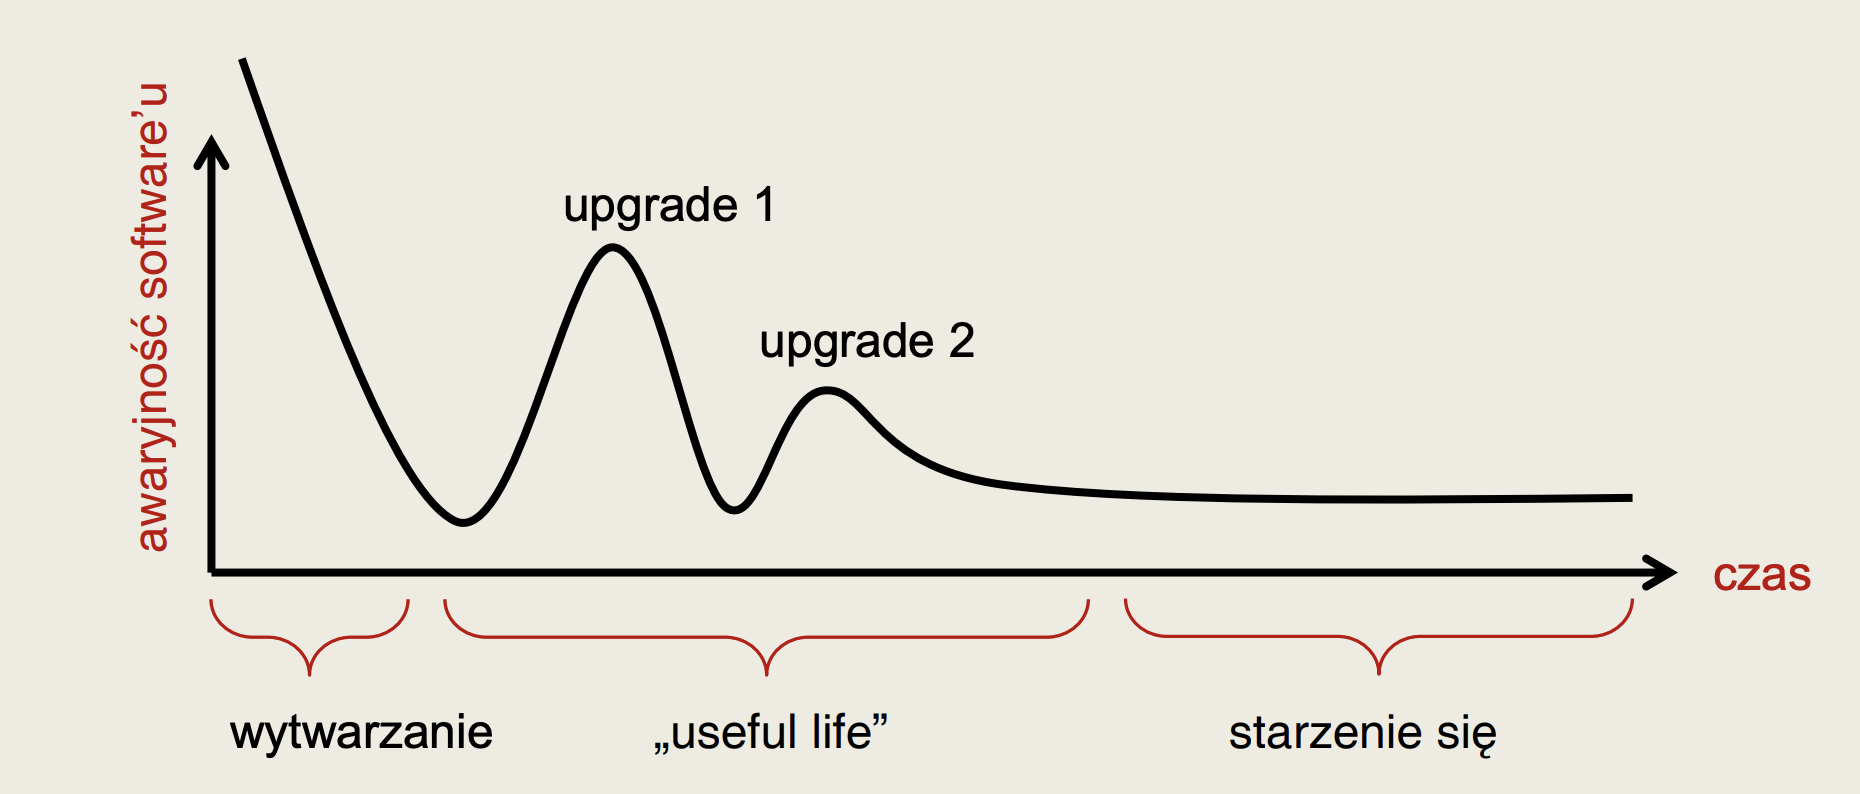
\includegraphics[width=\linewidth]{niezawodnosc.png}
    \end{figure}

    \begin{figure}[H]
        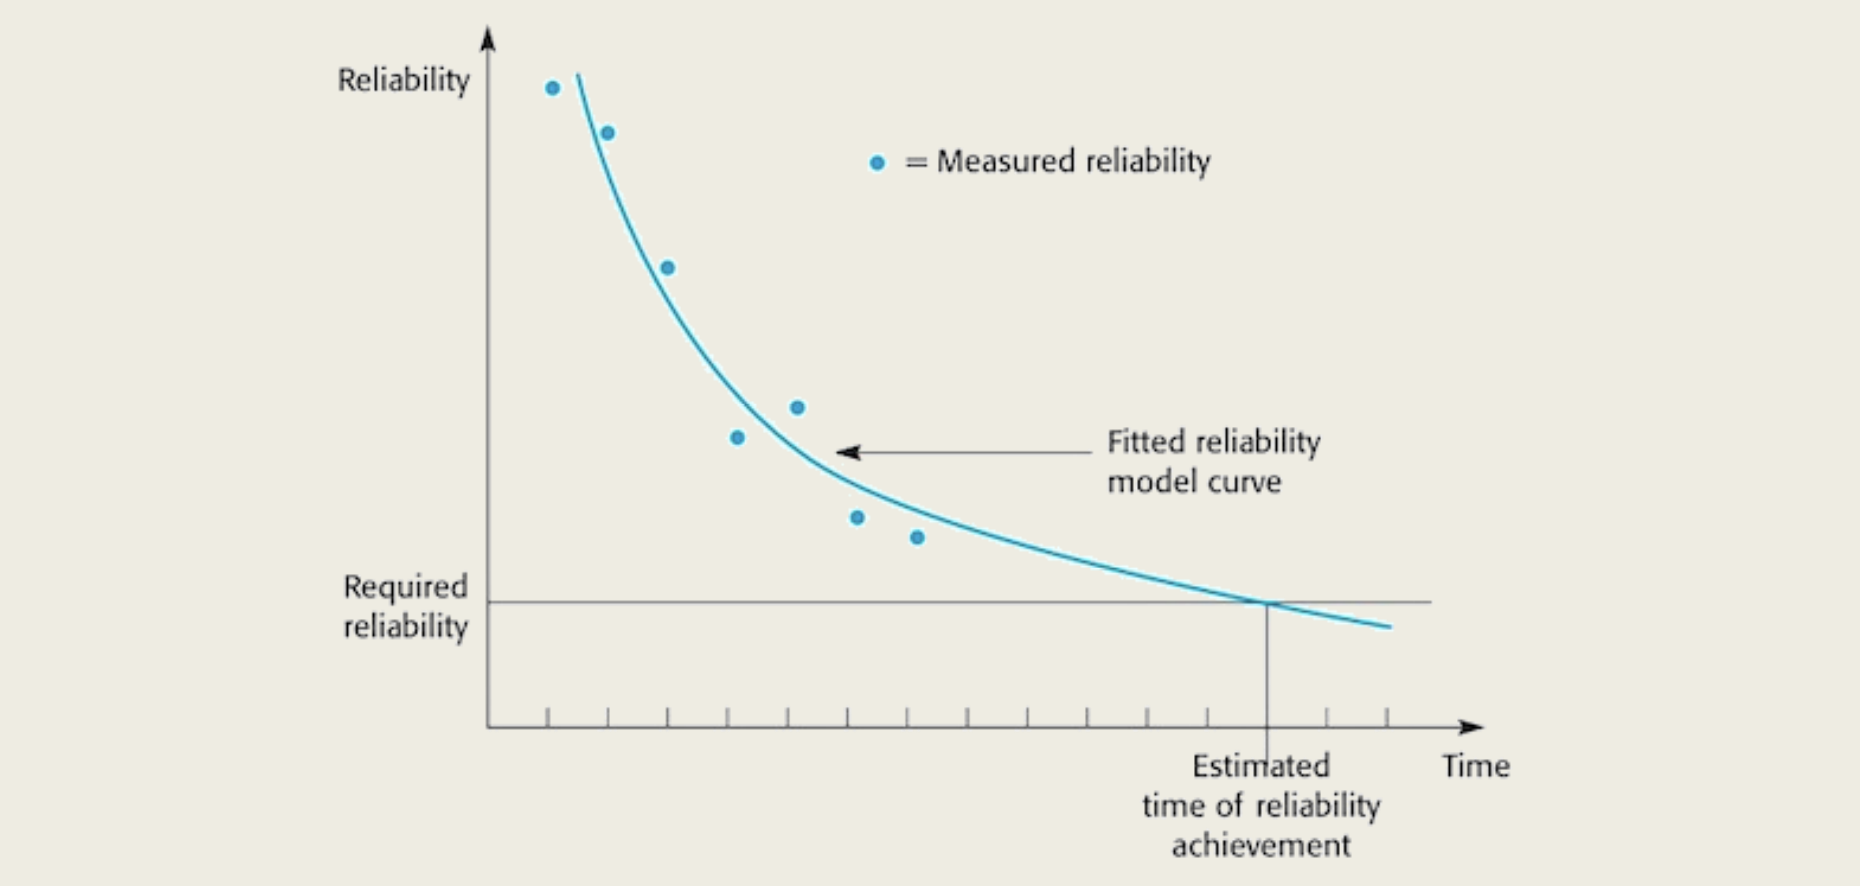
\includegraphics[width=\linewidth]{predniez.png}
    \end{figure}

    \subsubsection{Metryki}

    \begin{figure}[H]
        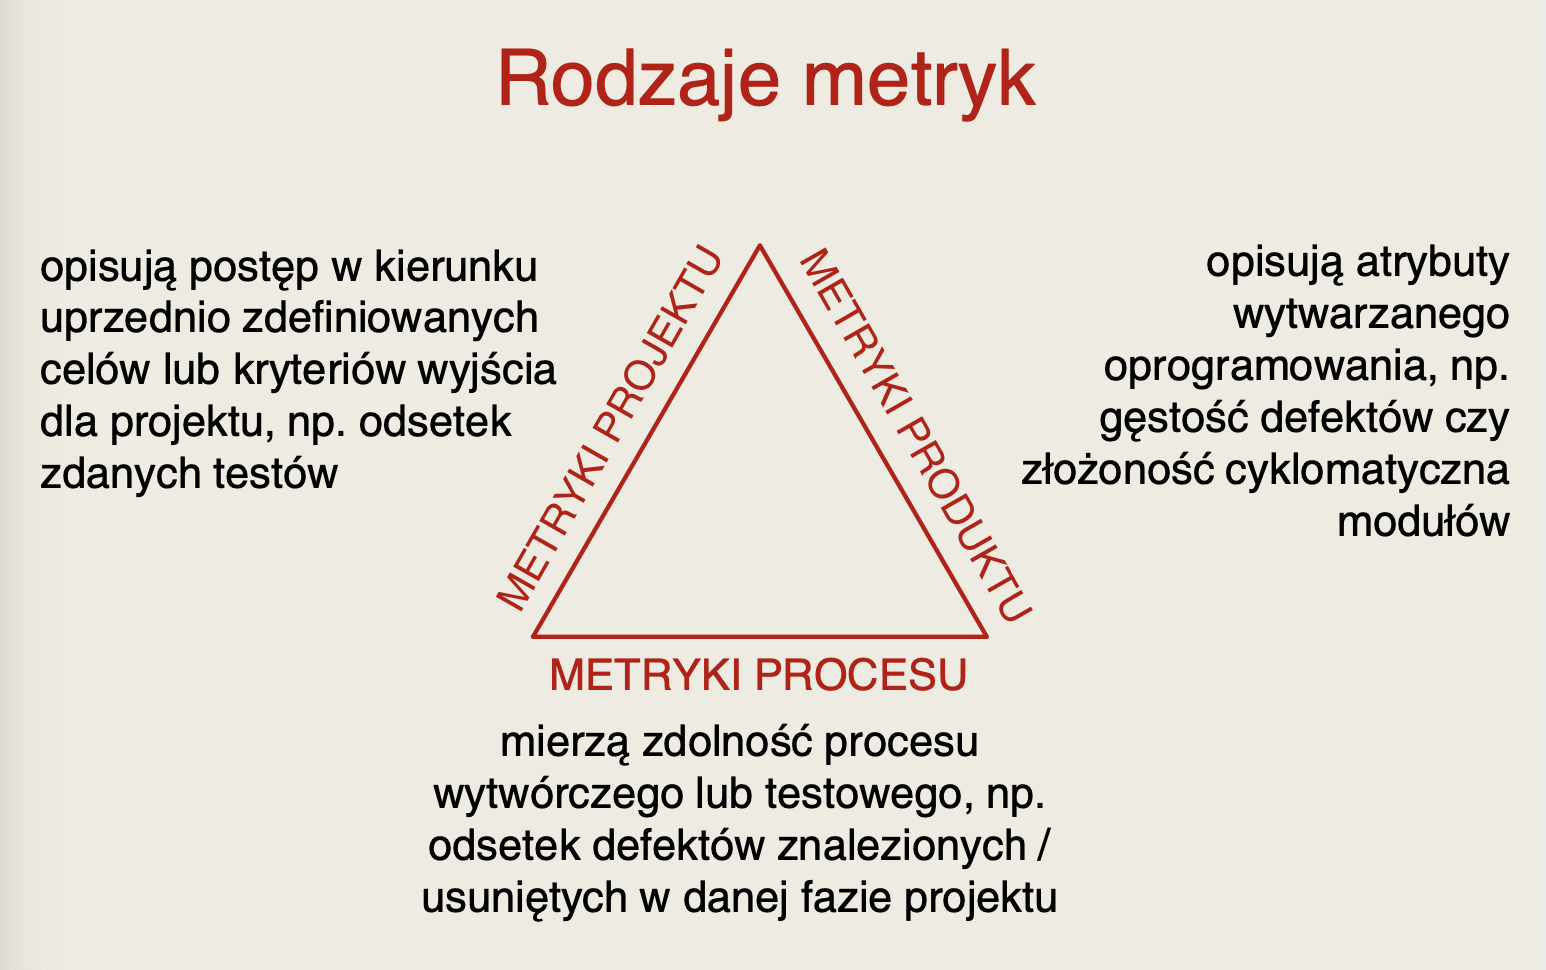
\includegraphics[width=\linewidth]{metryki.png}
    \end{figure}

    $MTTF$ = \textbf{Mean Time To Failure} - średni czas do awarii

    $MTTR$ = \textbf{Mean Time To Repair} - średni czas do naprawy

    $MTBF$ = \textbf{Mean Time Between Failures} - średni czas między awariami

    \begin{table}[H]
        \begin{center}
            \begin{tabular}{p{5cm} p{5cm} p{5cm}}
                \begin{align*}
                    MTTF = \frac{\sum_{i=1}^{N} OK_i}{N}
                \end{align*}
                &
                \begin{align*}
                    MTTR = \frac{\sum_{i=1}^{N} R_i}{N}
                \end{align*}
                &
                \begin{align*}
                    MTBF = MTTF + MTTR
                \end{align*}
            \end{tabular}
        \end{center}
    \end{table}
    Wraz ze wzrostem dojrzałości oprogramowania wzrasta MTTF.

    \subsubsection{Bezpieczeństwo}
    \begin{table}[H]
        \begin{center}
            \begin{tabular}{p{8cm} p{8cm}}
                \begin{itemize}
                    \item Bezpieczeństwo to zbiór atrybutów oprogramowania umożliwiający \textbf{ochronę przed nieautoryzowanym
                    dostępem} do programu i danych
                    \item Często \textbf{zagrożenia} bezpieczeństwa są \textbf{ukryte}, niejawne i niewidoczne
                    \item Błędy bezpieczeństwa często \textbf{nie mają widocznych symptomów} (nawet po włamaniu)
                    \item Profesjonalne testy bezpieczeństwa zwykle wykonywane przez zewnętrzne, \textbf{wyspecjalizowane} w tym obszarze \textbf{firmy}
                \end{itemize}
                &
                \begin{itemize}
                    \item \textbf{OWASP (Open Web Application Security Project} - obszerna baza zasobów dot. bezpieczeństwa webowego, np.:
                    \begin{itemize}
                        \item baza ataków
                        \item baza książek i innych materiałów o bezpieczeństwie
                        \item portal społecznościowy
                        \item projekty związane z bezpieczeństwem
                        \item dokumentacja, modele
                        \begin{itemize}
                            \item \textbf{SAMM (Software Assurance Maturity Model)} - model pozwalający organizacji zdefiniować i wdrożyć strategię dla zapewnienia bezpieczeństwa,
                            dopasowaną do określonych ryzyk
                        \end{itemize}
                    \end{itemize}
                \end{itemize}
            \end{tabular}
        \end{center}
    \end{table}

    \subsubsection{Użyteczność}
    \begin{itemize}
        \item Użyteczność to \textbf{zdolność systemu do bycia zrozumiałym}, łatwym do nauczenia i użycia oraz atrakcyjnym dla
        użytkownika
        \item Testowanie \textbf{skupia się na użytkownikach} i ich działaniu.
        \item \textbf{Efekty} testowania obserwowane na \textbf{prawdziwych}, końcowych \textbf{użytkownikach}, a nie testerach
        \item Testowanie użyteczności wymaga \textbf{wiedzy psychologicznej}, socjologicznej, z zakresu ergonomii, standardów dot.
        dostępności
    \end{itemize}

    \begin{table}[H]
        \begin{center}
            \begin{tabular}{p{8cm} p{8cm}}
                \textbf{Podcharakterystyki}
                \begin{itemize}
                    \item \textbf{Zrozumiałość} - jak łatwo zrozumieć co program robi i dlaczego mielibyśmy go używać?
                    \item \textbf{Łatwość nauki} - łatwość zrozumienia jak program działa
                    \item \textbf{Łatwość obsługi} - czy obsługa programu jest intuicyjna?
                    \item \textbf{Atrakcyjność} - czy użytkownik chętnie używa programu?
                \end{itemize}
                &
                \textbf{Metryki}

                Testowanie użyteczności jest ukierunkowane na pomiar:
                \begin{itemize}
                    \item \textbf{efektywności}
                    \begin{itemize}
                        \item np. stopień osiągnięcia przez użytkownika celów, z
                        określoną dokładnością i zupełnością
                    \end{itemize}
                    \item \textbf{wydajności}
                    \begin{itemize}
                        \item ilość zasobów zużytych do osiągnięcia celów, np. czas,
                        liczba kliknięć itp.
                    \end{itemize}
                    \item \textbf{satysfakcji} klienta z użytkowania produktu
                \end{itemize}
            \end{tabular}
        \end{center}
    \end{table}



    \begin{table}[H]
        \begin{center}
            \begin{tabular}{| p{8cm} | p{8cm} |}
                \hline
                \multicolumn{2}{|c|}{\textbf{TESTOWANIE UŻYTECZNOŚCI}} \\
                \hline
                \hline
                \multicolumn{2}{|c|}{\textbf{Proces}} \\
                \hline
                \textbf{Formatywne testowanie użyteczności} - przeprowadzane \textbf{iteracyjnie} w
                kolejnych \textbf{fazach projektowania} i prototypowania, aby ukierunkować
                (lub „uformować”) projekt poprzez identyfikację defektów użyteczności

                &
                \textbf{Całościowe testowanie użyteczności} - przeprowadzane \textbf{po implementacji}
                aby mierzyć użyteczność oraz identyfikować problemy z systemem
                lub komponentem traktowanym całościowo
                \\
                \hline
                \hline
                \multicolumn{2}{|c|}{\textbf{Rodzaje}} \\
                \hline
                \textbf{Formalne testowanie użyteczności} - często wymaga uprzedniego \textbf{przygotowania} rzeczywistych
                lub reprezentatywnych \textbf{użytkowników} (dostarczenie scenariuszy zadań, instrukcji)
                &
                \textbf{Nieformalne testowanie użyteczności} - pozwala użytkownikowi \textbf{eksperymentować} z
                oprogramowaniem, aby obserwatorzy ocenili jak trudna dla użytkownika jest praca z systemem \\
                \hline
                \hline
                \multicolumn{2}{|c|}{\textbf{Walidacja}} \\
                \hline
                \multicolumn{2}{|p{16cm}|}{powinna być przeprowadzona \textbf{w warunkach} tak \textbf{bliskich rzeczywistym} warunkom użytkowania
                oprogramowania, jak to tylko możliwe, np. w \textbf{laboratorium użyteczności}.} \\
                \hline
                \hline
                \multicolumn{2}{|c|}{\textbf{Wytyczne (guidelines)}} \\
                \hline
                \multicolumn{2}{|p{16cm}|}{są stosowane aby uzyskać \textbf{spójne podejście} do wykrywania i raportowania defektów
                użyteczności \textbf{na wszystkich etapach} cyklu życia. Powinny zawierać rzeczy takie jak:} \\
                \hline
                \begin{itemize}
                    \item dostępność instrukcji,
                    \item klarowność komunikatów,
                    \item \# kliknięć do ukończenia zadania,
                \end{itemize}
                &
                \begin{itemize}
                    \item komunikaty o błędach,
                    \item układ elementów na ekranie,
                    \item użycie kolorów, dźwięków itp.
                \end{itemize} \\
                \hline
                \hline
                \multicolumn{2}{|c|}{\textbf{Specyfikacja}} \\
                \hline
                \begin{itemize}
                    \item \textbf{Inspekcja, ewaluacja, lub przegląd}
                    \begin{itemize}
                        \item \textbf{Wymagania i specyfikacja}.
                        \item Heurystyczna ocena projektu GUI
                        \item Efektywniejsze, gdy UI jest bardziej widoczny, np. są screenshoty
                    \end{itemize}

                    \item \textbf{Weryfikacja i walidacja bieżącej implementacji}
                    \begin{itemize}
                        \item Weryfikacja przy pomocy \textbf{przypadków testowych}, czy oprogramowanie ma cechy użyteczności
                        zdefiniowane w wymaganiach
                        \item Walidacja przez scenariusze testowe(np. łatwość nauki)
                    \end{itemize}
                \end{itemize}
                &
                \begin{itemize}
                    \item \textbf{Dynamiczna interakcja z prototypami}
                    \begin{itemize}
                        \item Praca z \textbf{prototypami} i pomoc deweloperom w ich rozwijaniu
                        \item Prototypy mogą być przez uzyskanie realistycznego oglądu użytkowników
                    \end{itemize}

                    \item \textbf{Ankiety i kwestionariusze}
                    \begin{itemize}
                        \item Zbieranie \textbf{obserwacji} i \textbf{informacji zwrotnej} dotyczącej zachowania użytkowników
                        \item \textbf{SUMI} (Software Usability Measurement Inventory), \textbf{WAMMI} (Website Analysis and MeasureMent Inventory)
                        – standaryzowane benchmarki
                    \end{itemize}
                \end{itemize} \\
                \hline
            \end{tabular}
        \end{center}
    \end{table}

    \subsubsection{Wydajność}
    \begin{table}[H]
        \begin{center}
            \begin{tabular}{ p{8cm}  p{8cm} }
                \begin{itemize}
                    \item \textbf{Zdolność} oprogramowania do \textbf{zapewnienia odpowiedniej efektywności} w działaniu, relatywnie do
                    ilości zużytych zasobów
                    \item Systemy o znaczeniu krytycznym muszą dostarczać swoje funkcje w ściśle określonym czasie
                    \item Dla systemów czasu rzeczywistego (i innych) ważne jest \textbf{zużycie zasobów}.
                    \item Najczęstsza przyczyna błędów wydajności: \textbf{błędy projektowe} (a więc trudne do usunięcia w późniejszych fazach testów).
                \end{itemize}
                &
                \begin{itemize}
                    \item Testowanie wydajności powinno być przeprowadzane \textbf{na każdym etapie cyklu życia} – zwłaszcza w fazie projektu i kodowania.
                    \item \textbf{Błędy wydajności} powodują:
                    \begin{itemize}
                        \item wolny czas odpowiedzi
                        \item nieadekwatną przepustowość
                        \item problemy z niezawodnością (obciążenie)
                        \item nadmierne wymagania co do zasobów
                    \end{itemize}
                \end{itemize}
            \end{tabular}
        \end{center}
    \end{table}

    \begin{table}[H]
        \begin{center}
            \begin{tabular}{| p{8cm} | p{8cm} |}
                \hline
                \multicolumn{2}{|c|}{\textbf{Rodzaje testów} wydajności} \\
                \hline
                \begin{itemize}
                    \item testowanie \textbf{obciążenia}
                    \item testowanie \textbf{warunków skrajnych}
                    \item testowanie \textbf{skalowalności}
                    \item testowanie \textbf{wykorzystania zasobów}
                \end{itemize}
                &
                \begin{itemize}
                    \item testowanie \textbf{wytrzymałościowe}
                    \item testowanie \textbf{skokowe}
                    \item testowanie \textbf{niezawodności}
                    \item testowanie \textbf{z aktywnym tłem}
                    \item testowanie \textbf{punktu krytycznego}
                \end{itemize} \\
                \hline
                \hline
                \multicolumn{2}{|c|}{\textbf{Metryki} dla wydajności} \\
                \hline
                \begin{itemize}
                    \item \% wykorzystania procesora w kluczowym czasie
                    \item dostępna pamięć (RAM, wirtualna)
                    \item top N aktywnych procesów
                    \item liczba przełączeń kontekstów na sekundę
                \end{itemize}
                &
                \begin{itemize}
                    \item długość kolejek (procesor, dysk) w danym czasie
                    \item zużycie i wysycenie pamięci dyskowej
                    \item błędy sieci
                    \item czas podróży pakietu
                    \item czas prezentacji danych klientowi
                \end{itemize} \\
                \hline

            \end{tabular}
        \end{center}
    \end{table}

    \begin{figure}[H]
        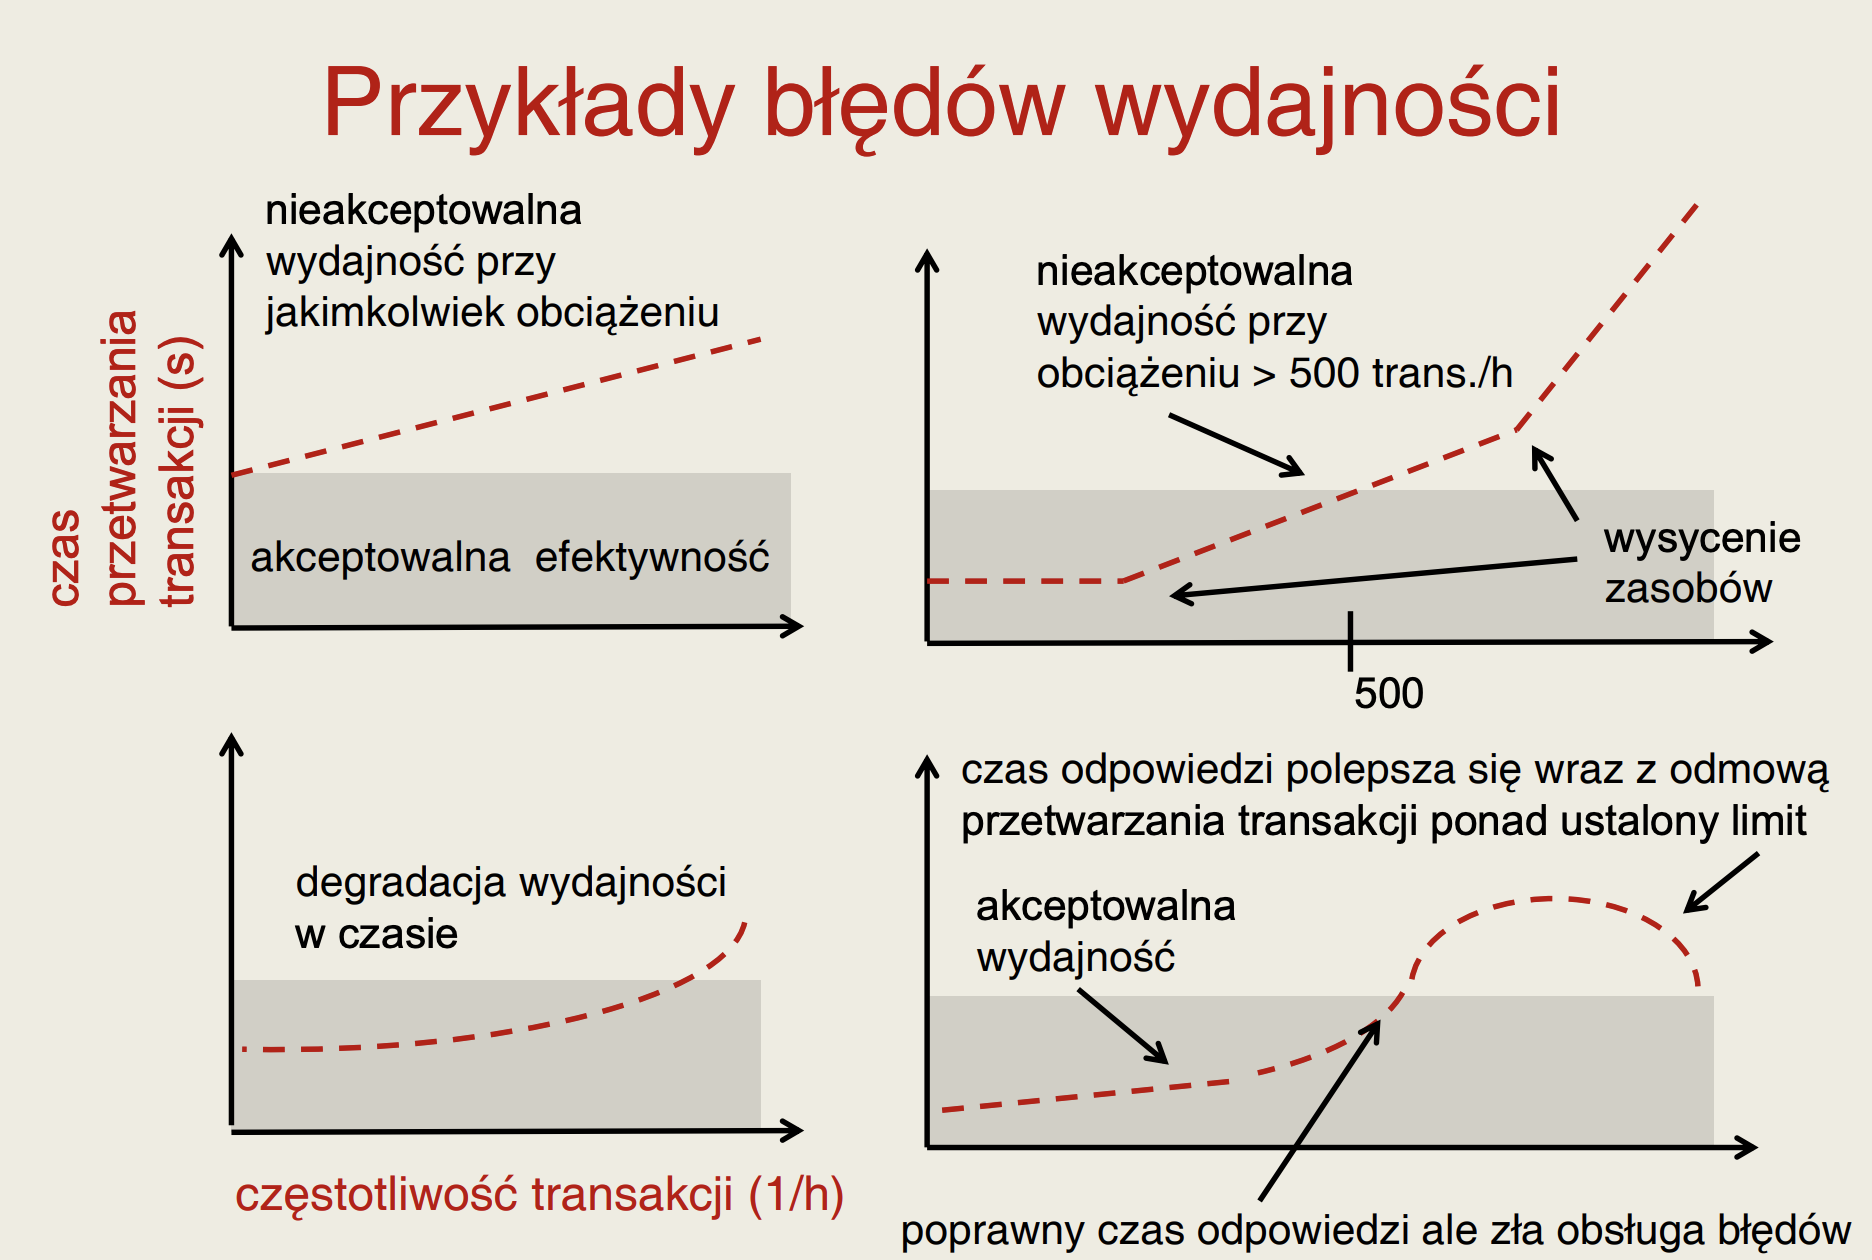
\includegraphics[width=\linewidth]{bledywyd.png}
    \end{figure}

    \subsubsection{Pielęgnowalność}
    \begin{itemize}
        \item Pielęgnowalność to \textbf{łatwość modyfikowania oprogramowania} w celu naprawy defektów, dostosowania do nowych
        wymagań, ułatwienia przyszłego utrzymywania lub dostosowania do zmian zachodzących w jego środowisku
        \item Oprogramowanie się nie zużywa, ale staje się \textbf{przestarzałe}.
        \item Zatem będą pojawiać się:
        \begin{itemize}
            \item nowe funkcjonalności
            \item patche
            \item aktualizacje oprogramowania
            \item nowe środowiska
        \end{itemize}
    \end{itemize}

    \begin{table}[H]
        \begin{center}
            \begin{tabular}{| p{8cm} | p{8cm} |}
                \hline
                \multicolumn{2}{|c|}{\textbf{Testowanie pielęgnowalności}} \\
                \hline
                \begin{itemize}
                    \item Defekty związane z pielęgnowalnością są powodowane m.in.:
                    \begin{itemize}
                        \item trudnym do zrozumienia kodem
                        \item zależnościami środowiskowymi
                        \item ukrytymi informacjami i stanami
                        \item złą architekturą
                        \item użyciem złej technologii
                    \end{itemize}
                \end{itemize}
                &
                \begin{itemize}
                    \item Zwykle nie przy pomocy skryptów testowych
                    \item Większość defektów jest \textbf{niewidoczna dla testowania dynamicznego}
                    \item Najlepiej sprawdzają się \textbf{techniki statyczne}
                \end{itemize} \\
                \hline
                \hline
                \multicolumn{2}{|c|}{\textbf{Podcharakterystyki pielęgnowalności}} \\
                \multicolumn{2}{|c|}{i \textbf{problemy} z nimi związane:} \\
                \hline
                \begin{itemize}
                    \item \textbf{Analizowalność} - łatwość diagnozowania problemów
                    \begin{itemize}
                        \item spaghetti code
                        \item brak dobrej dokumentacji
                        \item brak lub złe standardy/zalenia
                        \item abstrakcja kodu
                    \end{itemize}

                    \item \textbf{Modyfikowalność} - zdolność do wprowadzania zmian
                    \begin{itemize}
                        \item związanie (coupling)
                        \item brak kohezji
                        \item zły styl kodowania
                        \item kiepska dokumentacja
                    \end{itemize}
                \end{itemize}
                &
                \begin{itemize}
                    \item \textbf{Stabilność} - zdolność do unikania niespodziewanych efektów na skutek zmian
                    \begin{itemize}
                        \item związanie
                        \item brak kohezji
                        \item jakośc wymagań
                    \end{itemize}

                    \item \textbf{Testowalność} - łatwość walidacji po wprowadzonej zmianie
                    \begin{itemize}
                        \item brak lub zła dokumentacja
                        \item brak komentarzy w kodzie
                        \item antywzorce projektowe
                        \item zła konwencja nazewnictwa
                        \item brak instrumentacji kodu
                    \end{itemize}
                \end{itemize} \\
                \hline
            \end{tabular}
        \end{center}
    \end{table}

    \subsubsection{Przenaszalność}
    \begin{itemize}
        \item Przenaszalność to \textbf{łatwość, z jaką oprogramowanie może być przeniesione} z jednego środowiska do innego .
        \item Najczęstsze przyczyny problemów z przenaszalnością:
        \begin{itemize}
            \item zależności środowiskowe
            \item zajmowanie zasobów
            \item niestandardowe interakcje systemu operacyjnego
        \end{itemize}
    \end{itemize}

    \begin{table}[H]
        \begin{center}
            \begin{tabular}{| p{8cm} | p{8cm} |}
                \hline
                \multicolumn{2}{|c|}{\textbf{Podcharakterystyki przenaszalności}} \\
                \hline
                \begin{itemize}
                    \item \textbf{Adaptowalność} – zdolność do adaptacji w innym środowisku bez
                    podejmowania akcji innych niż przewidziane w tym celu – nie zawsze dobre; nie zawsze tanie i proste (Java)
                    \item \textbf{Zastępowalność} – możliwość do bycia zastąpionym przez inny
                    produkt do tego samego celu w tym samym środowisku – np. DLL, COM, DCOM, COTS…
                \end{itemize}
                &
                \begin{itemize}
                    \item \textbf{Instalowalność} – możliwość bycia zainstalowanym w danym środowisku
                    – zależności, błędy, niemożność przerwania…
                    \item \textbf{Koegzystencja} – zdolność do współistnienia z innym, niezależnym oprogramowaniem dzielącym środowisko
                    – np. „przywłaszczenie” standardowego skrótu klawiszowego lub kombinacji dla znaków specjalnych przez inny program
                \end{itemize} \\
                \hline
            \end{tabular}
        \end{center}
    \end{table}
\end{document}